\documentclass{bioinfo}
\usepackage{url}
\usepackage{comment}

\usepackage[british,english]{babel}
\usepackage{mathpazo}
\usepackage{color}
\definecolor{deepblue}{rgb}{0,0,0.5}
\definecolor{deepred}{rgb}{0.6,0,0}
\definecolor{deepgreen}{rgb}{0,0.5,0}
\definecolor{white}{rgb}{1,1,1}

\usepackage{listings}
\usepackage{setspace}

\definecolor{Code}{rgb}{0,0,0}
\definecolor{Decorators}{rgb}{0.5,0.2,0.2}
\definecolor{Numbers}{rgb}{0.5,0,0}
\definecolor{MatchingBrackets}{rgb}{0.25,0.5,0.5}
\definecolor{Keywords}{rgb}{0,0.6,0}
\definecolor{self}{rgb}{0,0,0}
\definecolor{Strings}{rgb}{0.6,0.,0}
\definecolor{Comments}{rgb}{0,0.63,1}
\definecolor{Backquotes}{rgb}{0,0,0}
\definecolor{Classname}{rgb}{0,0,0}
\definecolor{FunctionName}{rgb}{0,0,0}
\definecolor{Operators}{rgb}{0,0,0}
\definecolor{Background}{rgb}{1,1,1}
\definecolor{Modules}{rgb}{0,0,0.8}

\lstnewenvironment{python}[1][]{
\lstset{
%numbers=left,
numberstyle=\footnotesize,
numbersep=1em,
xleftmargin=0em,
framextopmargin=2em,
framexbottommargin=2em,
showspaces=false,
showtabs=false,
showstringspaces=false,
%frame=l,
tabsize=4,
% Basic
basicstyle=\ttfamily\footnotesize\setstretch{1},
backgroundcolor=\color{Background},
language=Python,
% Comments
commentstyle=\color{Comments}\slshape,
% Strings
stringstyle=\color{Strings},
morecomment=[s][\color{Strings}]{"""}{"""},
morecomment=[s][\color{Strings}]{'''}{'''},
% keywords
morekeywords={import,from,class,def,for,while,if,is,in,elif,else,not,and,or,print,break,continue,return,True,False,None,access,as,del,except,exec,finally,global,import,lambda,pass,print,raise,try,assert},
keywordstyle={\color{Keywords}\bfseries},
% additional keywords
morekeywords={[2]@parametric},
keywordstyle={[2]\color{Decorators}\slshape},
emph={self},
emphstyle={\color{self}\slshape},
%
}}{}


\usepackage[T1]{fontenc}
% \usepackage[latin9]{inputenc}
\usepackage{float}
\usepackage{amsmath}
\usepackage{graphicx}
\usepackage{setspace}
\usepackage{amssymb}
\usepackage{natbib}
\usepackage[title]{appendix}
\usepackage{siunitx}
\usepackage{chngcntr}
\usepackage{algorithmic}
\renewcommand{\algorithmicrequire}{\textbf{Input:}}
\renewcommand{\algorithmicensure}{\textbf{Output:}}

\usepackage{multirow}
\usepackage{rotating}
%\usepackage{xcolor}
\usepackage[pdfborder={0 0 0}]{hyperref}
%\usepackage{units}

% This one seems to break formatting of top page
% \usepackage{multicol}

\usepackage{widetext}

\graphicspath{{Figures/}}

\lstset{language=python,
	basicstyle=\ttfamily,
	extendedchars=true,
	xleftmargin = 0pt,
	% rulecolor=\color{black!50},
        aboveskip = 0.5ex,
        belowskip = 0.6ex,
	%escapebegin={\color{green!50!black}},
	%commentstyle=\slshape\color{green!50!black},
	%stringstyle=\rmfamily\color{blue},
	showstringspaces=false,
	tabsize=2,
	breaklines=true,
        morekeywords={{,},=,:},
        frame=single,xleftmargin=\fboxsep,xrightmargin=-\fboxsep
    }


\makeatletter
\newfloat{algorithm}{H}{loa}[section]
\floatname{algorithm}{Algorithm}
\counterwithout{algorithm}{algorithm}
\def\argmin{\mathop{\operator@font arg\,min}}
\def\argmax{\mathop{\operator@font arg\,max}}
\makeatother

\copyrightyear{}
\pubyear{}

\begin{document}
\firstpage{1}

\title[nipy-paper]{Analysis of functional imaging data with NIPY}

\author[Roche,Thirion,Varoquaux,Taylor,Brett]
{Alexis~Roche\,$^{1,2,}$, Bertrand~Thirion\,$^{3}$, Ga\"el~Varoquaux\,$^{3}$,
Jonathan~Taylor\,$^{4}$, Matthew~Brett\,$^{5}$\footnote{to whom correspondence
should be addressed. e-mail: matthew.brett@gmail.com} and NIPY
contributors $^{6}$}

\address{\,$^{1}$University Hospital, Lausanne, Switzerland\\
  \,$^{2}$Siemens Healthcare Sector, Lausanne, Switzerland\\ 
  \,$^{3}$INRIA, Parietal team, Neurospin, Saclay, France\\
  \,$^{4}$Stanford University, Stanford, CA, USA\\
  \,$^{5}$University of California, Berkeley, CA, USA\\
  \,$^{6}$\texttt{https://github.com/nipy/nipy/contributors}
}

\history{}

\editor{}

\maketitle

\begin{abstract}
\noindent

NIPY is a library and application for analyzing functional imaging data.   We
intended the project to be a project open to anyone who wanted to contribute
high-quality code.  Our aim is to make it easier for researchers to understand
the analysis and build their own tools, by writing code that is clear,
well-adapted to the scientific problem, and fast enough to run in reasonable
time.

Using Python has made it easier for us to work together because of the
readability of the language, the popularity of the language among
open-source developers, and Python's emphasis on testing and
documentation.

The package developed from a collaboration between researchers in Stanford,
Berkeley and INRIA/CEA, Neurospin in France.

Notable features of the NIPY package are: scriptable image diagnostics
including flexible PCA; combined slice-timing and movement correction
for functional MRI images; flexible registration model with pluggable
cost functions and optimization algorithms; common spatial models of
function encountered in neuroimaging (cluster-level models;
parcellations); fast and flexible specification of regression models
within and across subjects and groups; visualization of statistical
brain maps in 2D and 3D.

We will describe these features of the package with examples of their use.

\section{Keywords:} Python, functional MRI, structural MRI, 
Deconvolution, Medical imaging, Open source software, Deterministic
tractography, Probabilistic tractography, Visualization.

\end{abstract}

\section*{Skeleton}

This section will be removed later on. Let's have it for now to
clarify the paper outline for every author. Here is a possible
outline, please feel free to modify:

\begin{verbatim}
Introduction
  Philosophy/Mission
  General Design Aspects
File Formats 
Preprocessing
   Image diagnostics
   Spatiotemporal realignment
   Generic image registration
Statistical analysis
   GLM specification/estimation
   Cluster-level analysis
   Parcel-based Bayesian analysis
Visualization
Conclusions
\end{verbatim}

\section{Introduction}

Someone will write this.

\section{File formats}

\section{Preprocessing}

\subsection{Image diagnostics}

\subsection{Spatiotemporal realignment}

FMRI sequences present spatio-temporal distortion due to the
combination of head motion during scanning and staggered slice
acquisition. While most fMRI processing packages provide tools to
correct for motion and slice timing separately, a common dilemma is to
determine which correction should be applied first. NIPY proposes a
four-dimensional realignment algorithm to perform both tasks
simultaneously \citep{roche:tmi:11}. This approach makes it possible
to account and correct for {\em continuous} movements that occur
throughout image acquisition. In addition, the method limits the
effect of BOLD signal changes on realignment \citep{freire:ni:01} by
using an adaptive reference image.

Spatiotemporal registration is implemented by a class called {\tt
  SpaceTimeRealign} which takes as initialization arguments a list of
four-dimensional images corresponding to successive fMRI runs for a
particular subject, and image acquisition information (inter-scan
repetition time, slice acquisition times, acquisition plane). Rigid
motion estimation is performed within each run as well as between
runs. Once motion parameters are estimated, it is possible to resample
each run on a regular four-dimensional lattice, thereby reconstructing
fMRI runs corrected for motion and slice timing effects. Note that
this algorithm does not rely on a particular BOLD response model, and
is therefore applicable, in principle, to both stimulation and resting
state fMRI.

\subsection{Generic image registration}

NIPY has a generic module ({\tt algorithms.registration}) that
implements the registration of two three-dimensional images as the
numerical maximization of a registration measure with respect to a
spatial transformation set. The module is designed to enable the user
to customize both the registration measure and the transformation set,
either by choosing among pre-defined classes or by plugging external
classes. Built-in registration measures include mutual information
\citep{maes:tmi:97}, normalized mutual information
\citep{studholme:pr:98}, standard correlation and correlation ratio
measures \citep{roche:ijist:00}. Built-in transformation sets include
rigid, similarity and 12-parameter affine transformations, and we are
currently developing diffeomorphic nonrigid transformation classes.





\section{Statistical analysis}

\subsection{GLM specification/estimation}
% Bertrand
% - Design matrix computation: Simplicity of the interface
% - Idem for GLM
% - uncoupling GLM / contrasts

FMRI data analysis relies on the modeling of temporal effects that
represent the expected impact of the experimental events on the brain
signals, plus a set of confounds.
%
Neuroimagers typically have to make a set of choices here: for
instance, they need to decide which model of the hemodynamic response
function (hrf) they want to use to model evoked response. 
%
The hrf is a low-pass filter that delays some input signal --an
idealized model of neural responses-- with the observed Blood
Oxygen-Level Dependent (BOLD) contrast.
%
Different parametrization of this filter have been proposed in the
literature \cite{Friston1998,Glover1999}; moreover, it is often
advised to include the first derivative of the chosen model to account
for unpredictable delays in the response, that can be due to local
vasculature differences, uncertainty on the exact neural response
timing, or shortcomings of the slice timing correction.
%
Similarly, several different parametrizations can be used to model
signals of no interest, such as low-frequency drifts.
%
In practice, it is advised to consider different parametrizations of
the expected responses.
% 
In terms of software design, this means that as simple yet flexible
interface is needed for model specification
%% Provide here a snippet of code and an example
See for instance the listing \ref{dmtx} and the result in
Fig. \ref{fig:dmtx}

\lstset{language=Python,caption={Creation of a design matrix with
    nipy}, label=dmtx}
\begin{widetext}
\lstinputlisting{dmtx.py}
\end{widetext}
\begin{figure}
\begin{center}
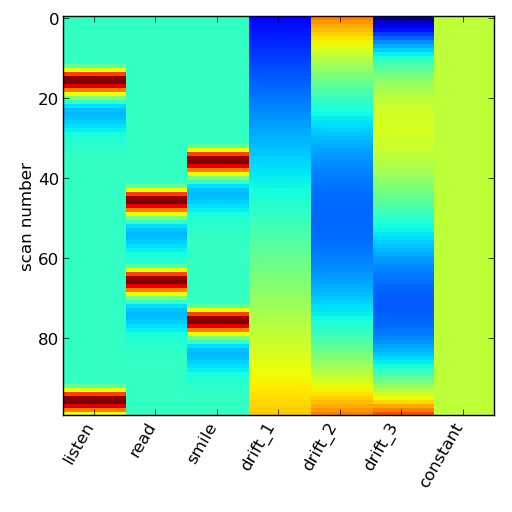
\includegraphics[width=.8\linewidth]{dmtx.png}
\end{center}
\caption{ Result of listing 1: the design matrix contains columns that
  contains the ideal response to input stimuli and a basis of
  polynomial function to model temporal drifts.}
\label{fig:dmtx}
\end{figure}


General Linear Model fitting consists then in estimating the brain
responses associated with the columns of design matrix.
%
The fit consists in a weighted least-square fit to estimate the model
parameters and a variance-covariance matrix parametrized by two
parameters: the amount of noise variance in the voxel time course and
the lag-1 autocorrelation of the noise \cite{Bullmore1996}. 
%
The model and covariance parameters are estimated in an alternate
optimization scheme.
%
The corresponding interface is relatively simple, as the user simply
needs to provide the design matrix and the data matrix. 
%
It yields a class that contains summary statistics (estimated effects
and their covariance matrix) that can be used for further
investigation; the standard way of exploiting this output consists in
specifying a linear combination of the regressors and test the
significance in signed (t-) or unsigned (F-test)
%
The simplicity of the illustrated in listing \ref{glm}.

\lstset{language=Python, caption={Run of a GLM, based on the
    previously defined design matrix, on a simulated dataset. The
    FMRILinearModel object takes images as input and returns a result
    object, that, when given a certain linear contrast, returns a
    nibabel.Nifti1Image that yields the z-variate corresponding to the
    p-value of a positive effect in each voxel of the dataset.},
  label=glm}

\begin{widetext}
\lstinputlisting{glm.py}
\end{widetext}

The z- or equivalently p-variates can then easily be corrected for
multiple testing using a Bonferroni procedure or a False discovery
rate correction.

\subsection{Group analysis and statistics}
Nipy contains also some tools for linear group statistics: these
statistics consist in estimating the impact of subjects-related
information described in a design matrix (such as the age, some
behavioral score or the membership a group of control or patient
subject).
%
The same API used in the first-level GLM can be used in the second
glm; moreover, it can take into account the uncertainty on the first
level effects, yielding the so-called mixed-effects model \cite{Roche2007}.
%
Intuitively, such a model plays a useful role at down-weighting
observations that are estimated with larger uncertainty during the
first-level GLM.
%
The output of such a test is typically a log-likelihood ratio test.
The significance of such a statistic is hard to assess from the data
(although it can usually be safely approximated by a Student variable
with a number of degrees of freedom corresponding to those of the
second-level model).
%
Another possibility is to run a permutation test. No simple mechanism
has been set up to do so at present in nipy, but this will probably be
added in the future.
%
Note that in some simple cases (one- or two-sample tests) a
permutation procedure is easily handled in Numpy.
%
%More complex models, however, require some caution.

\subsection{Cluster-level analysis}


\subsection{Parcel-based Bayesian analysis}

A weakness of conventional mass-univariate group analysis is that it
relies on averaging imperfectly aligned multi-subject data, thereby
mixing signals from potentially different functional
areas. Cluster-level inference can be used to mitigate this problem,
but comes at the price of sacrificed localization power. NIPY
implements an alternative group inference method using a hierarchical
statistical model that explicitly incorporates spatial uncertainty
in the standard space, and performs an approximate Bayesian inference
on group effects assumed to be piecewise constant within the brain
according to a given, user-supplied parcellation
\citep{keller:sinica:08,keller:miccai:09}. 

The method is implemented by NIPY's {\tt ParcelAnalysis} class, which
typically runs in seconds owing to a fast expectation-propagation
scheme \citep{minka:techrep:05} used to carry out approximate
inference. An example of use is provided in
Figure~\ref{fig:parcel_group}, left panel, where we infer the effect
of changing the speaker for different sentences in an auditory fMRI
experiment from 15 {\em non-smoothed} first-level contrast images. We
use the AAL atlas \citep{tzourio:ni:02} as the underlying parcellation
in this example. The method highlights the inferior temporal gyri and
the left para-central lobule as the regions with strongest
effects. Note that it is possible to switch off the localization
uncertainty model and replace it with conventional image smoothing, as
shown in the right panel of Figure~\ref{fig:parcel_group}. We then
obtain more regions with strong effects, but this likely is an
artefactual effect of smoothing.

\begin{figure}
\begin{center}
  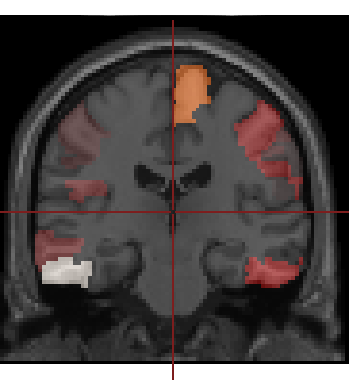
\includegraphics[width=0.23\textwidth]{parcel_group_analysis.png}
  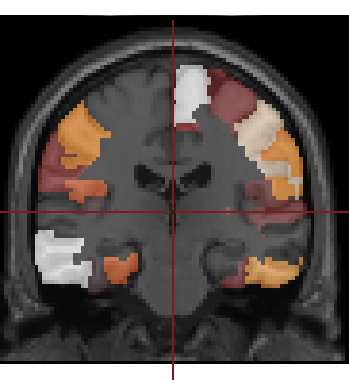
\includegraphics[width=0.23\textwidth]{parcel_group_analysis_naive.png}
\end{center}
\caption{Parcel-based Bayesian estimation of BOLD effects at
  population level for a speaker effect in an auditory fMRI
  experiment. Left, using a model of localization uncertainty in MNI
  space; right, using conventional image smoothing
  (FWHM=8mm). Brighter colors indicate larger estimated effects.}
\label{fig:parcel_group}
\end{figure}

\subsection{Brain Functional landmarks}
% Bertrand

Besides standard group analysis, that performs a probabilistic
rejection of the null hypothesis that the cross-subject average signal
is zero at any position of the brain volume, another possibility
consists is finding in which region of the brain active spots tend to
be concentrated.
%
Such regions can be called \textit{Brain Functional landmarks},
meaning that they display a pattern of activation that can be found
reliably in a significant fraction of the population.
% 
Identifying such brain functional landmarks entails two operations:
the first one is to define what an active patterns is in practical
terms. The second one consists in deriving a model of the distribution
of these patterns in the domain of interest.

The definition of active patterns, often colloquially referred to as
\textit{blobs} can easily be performed by using a variant of the
watershed algorithm on each activation maps, that separates the peaks
of activation above a certain thresholded, provided that the resulting
regions are large enough (e.g. 10 voxels at least).
%
Note that this is slightly more involved than more traditional
neuroimaging approaches that merely consider the connected components
of supra-threshold regions as structures of interest.
%
The corresponding algorithm is illustrated in Fig. \ref{fig:watershed}.

\begin{figure}
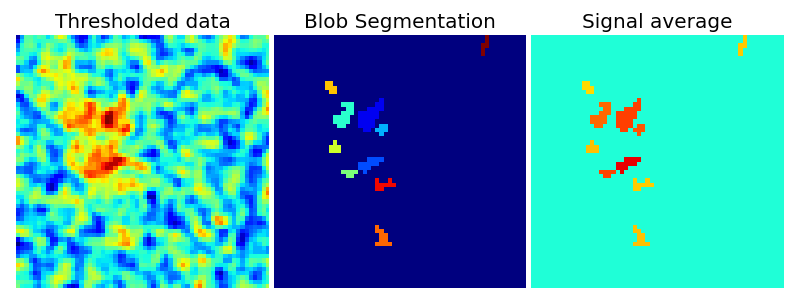
\includegraphics[width=\linewidth]{Figures/blob}
\caption{Segmentation of the blobs of an image. The regions the input
  image (left) above a given threshold are separated into blobs
  (middle). This amounts to deriving a sketchy representation of the
  input (right) that retains peak values on a flat background.}
\label{fig:watershed}
\end{figure}

The most important and difficult part consists in deriving a spatial
distribution of these blobs, in order to identify in which regions of
the domain of interest they are found.
%
this assumes that the data have already been put in a common coordinate
system.
%
We decided to introduce a class of probabilistic distribution,
Dirichlet Process Mixture Models, aka infinite Gaussian mixture
models, that give a lot of flexibility to model distributions of the
coordinates of active regions across individuals: the shape of the
modes can be relatively arbitrary, while the unlimited number of nodes
accounts for deviations from the normality of the model.
%
After convergence of the density estimate, the modes can be isolated,
are taken as a tag of homologous regions across individuals.
%
However, the model also includes a null component, which is a uniform
distribution over the domain of interest, that models the occurrence of
false positives in the initial pattern extraction step.
%
The final set of landmarks reflects thus a statistical decision on
the regions of the domain in which strong effects are observed.
%
This approach, somewhat reminiscent of recent meta-analysis frameworks,
has been described in detail in \cite{Thirion2007} and
\cite{Thirion2010}.
%
In particular it has been shown that such landmarks better predict
the occurrence of active regions in left-out subjects that classical
random- or mixed-effects analysis models.
%
This approach is illustrated in Fig. \ref{fig:landmarks} 

\begin{figure}
\begin{center}
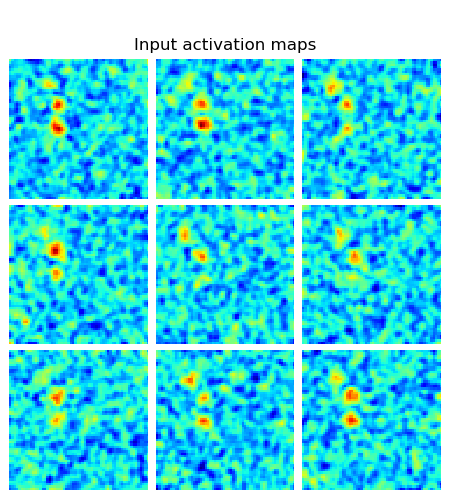
\includegraphics[width=\linewidth]{Figures/bsa_inputs.png}
{\Huge $\Downarrow$}
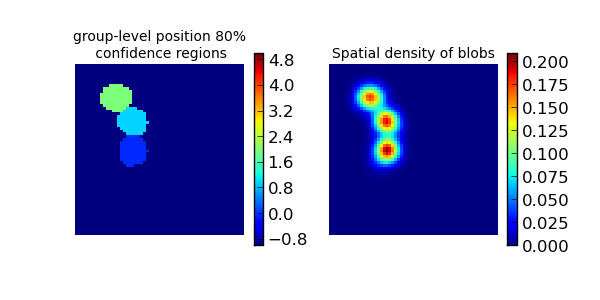
\includegraphics[width=\linewidth]{Figures/bsa_results.png}
\end{center}
\caption{Illustration of the Functional landmarks approach. (Top) a
  set of individual activation maps are provided as input to the
  methods, together with a threshold. (Bottom) The algorithm estimates
  the spatial distribution of the resulting activation patterns
  (blobs) and separates them into modes.}
\label{fig:landmarks}
\end{figure}

\section{Visualization}
% Gael or Bertrand
Non-interactive visualization tools are available in Nipy, based
either on Matplotlib or Mayavi libraries.
%
These tools are mostly helpers that make it easy to overlay an
activation image on the T1 image of that subject or on a T1 template
in MNI space.
%
The images can be sliced in any direction and a set of orthographic
views according to three directions can be obtained.
%
An important feature of the proposed approach is that the two images
overlayed do not need to be sampled with the same field of view or
resolution: they get resampled internally when needed. 
%
This is made possible by providing the affine transform that maps the
images to some (implicit) reference space: the MNI space or the
individual anatomical space.

\lstset{
  language=Python,caption={Vizualization of an activation image}, label=viz}

% \begin{widetext}
\noindent
\hspace*{-.5cm}
\lstinputlisting{viz_short.py}
% \end{widetext}
\begin{figure}
\begin{center}
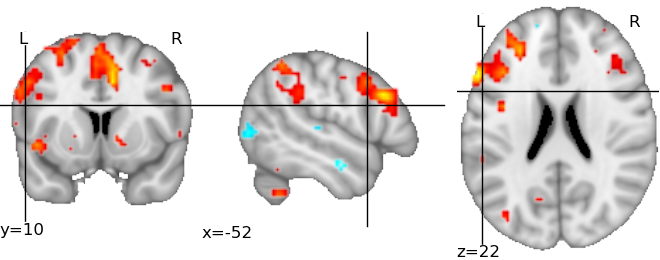
\includegraphics[width=\linewidth]{Figures/ortho_view.png}
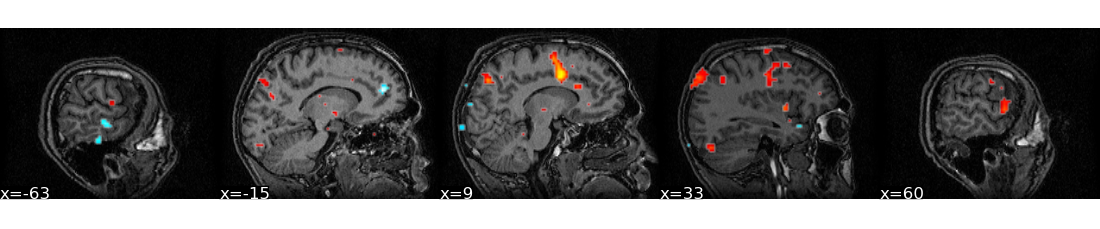
\includegraphics[width=\linewidth]{Figures/x_view.png}
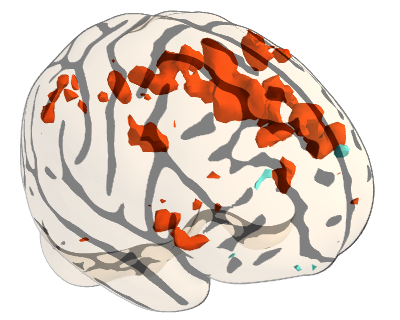
\includegraphics[width=.6\linewidth]{Figures/viz_3d.png}
\end{center}
\caption{Visualization of an activation image (top) Result of listing \ref{viz} A brain activation image is
  overlayed on MNI template, thesholded at z=3; note that the image
  was dynamically resampled from 3 to 1mm isotropic resolution.
(middle) the activation is overlayed on the anatomical image of the subject, with a black background, and sliced in the sagittal orientation.
(bottom) A 3D view obtained with the nipy.labs.viz.plot\_map\_3d module}
\label{fig:viz}
\end{figure}

Similarly, slices of the images according to the sagittal, coronal or
axial directions can be obtained.

It is also possible to obtain 3D views, through an (optional)
dependence on Mayavi. Note that in that case the activation blobs are
overlayed on a template.
%
The API is as simple as for 2D views.


\section{Conclusion}


\section*{Acknowledgments}
Whom do we need to acknowledge?

\section*{Disclosure/Conflict-of-Interest Statement}
Is it true that there are no conflicts of interest relating to this
work?


\begin{comment}
\section*{Formatting stuff}

To be removed later on.

This is to show how graphics (EPS) files are included. We use EPS for
speed. The first one is spread across both columns, and the second one
is just in a single column:

\begin{figure*}
%\centerline{\includegraphics[width=160mm]{Figures/Fig_4_cst_simplification_relabeled_triple.eps}}
\caption{This is the figure caption - and a label to refer to it in the text \label{Fig:big_picture}}

\end{figure*}

When we want to refer to this figure we use the label (see
Fig.~\ref{Fig:big_picture}).


Here are some displayed equations (see Eq.~\ref{eq:direct_flip_distance}):
\begin{eqnarray}
  d_{\textrm{direct}}(s, t) = d(s, t) & = & \frac{1}{K}\sum_{i=1}^{K}|s_{i}-t_{i}|,\nonumber\\
  d_{\textrm{flipped}}(s, t) & = & d(s,t^F) = d(s^F,t),\nonumber\\
  \textrm{MDF}(s, t) & = & \min(d_{\textrm{direct}}(s, t), d_{\textrm{flipped}}(s, t))\label{eq:direct_flip_distance}.
\end{eqnarray}

Inline mathematics goes like this: $\frac{1}{K}\sum_{i=1}^{K}|s_{i}-t_{i}|$

Here we have an example of a table (see Table~\ref{Table_1}).

\begin{table}[th] \processtable{QB centroids performance compared with
random subsets\label{Table_1}} {\begin{tabular}{rrrr} %\hline Thresholds &
Comparison & Coverage \% (s.d.) & Overlap (s.d.) \\ \hline
\multirow{2}{*}{$10$~mm/$10$~mm} & QB Centroids & 99.96 (0.007) & 2.44
(0.08)\\ & Random & 90.49 (0.41) & 6.16 (0.55)\\ \hline
\multirow{2}{*}{$20$~mm/$20$~mm} & QB Centroids & 99.99 (0.004) & 3.54
(0.18)\\ & Random & 95.86 (0.62) & 6.81 (0.93)\\ \hline
\end{tabular}}{}
\end{table}
\end{comment}

%%\selectlanguage{british}%
\bibliographystyle{apalike2}
%\bibliographystyle{plainnat}
%\bibliographystyle{IEEEabrv, IEEEtran}
%\bibliographystyle{IEEEtran}
%\bibliographystyle{elsarticle-harv}
\selectlanguage{english}
\bibliography{nipy_paper}

\end{document}
